\section{مقدمه}

%\begin{frame}{پردازش ابری}
%	تعریف پردازش ابری ...
%\end{frame}

\begin{frame}{اهمیت پردازش ابری}

ارائه خدمات ابری باعث رشد پیشرفت در علم و صنعت شده است.

\begin{itemize}\RTList
\فقره \مل{CERN} به کمک خدمات ابری گوگل چندین پتابایت داده را در سال پردازش می‌کند\مرجع{google_cern}.
\فقره تمام زیرساخت \مل{Netflix} از خدمات آمازون است\مرجع{amazon_netflix}.
\فقره شرکت \مل{Micros} از خدمات آمازون برای پویانمایی فیلم‌ها استفاده می‌کند\مرجع{amazon_mikros}.
\end{itemize}
\end{frame}

\begin{frame}{ویژگی پردازش ابری}
	در خدمات ابری دو مورد زیر اهمیت بسزایی دارند.
	\begin{itemize}\RTList
		\فقره مقایس‌پذیری
		\فقره اتکاپذیری
	\end{itemize}
	\pause
	\begin{center}
		\mybox{راهکار}{
	استفاده از معماری‌های توزیع‌شده مانند \توچشم{میکروسرویس} راهکار مورد استفاده
	در عمل برای رسیدن به این دو مورد است\مرجع{baboi2019dynamic}.	}		
	\end{center}
\end{frame}

\begin{frame}{معماری میکروسرویس}
	\begin{itemize}\RTList
	\فقره در این معماری، سیستم به مولفه‌هایی ریزدانه‌ و مستقل تقسیم می‌شود.
	\فقره موله‌ها با یک دیگر در بستر شبکه‌های کامپیوتری در ارتباط هستند.
	\فقره هر مولفه می‌توانند به صورت جداگانه بر روی تعدادی خدمت‌رسان اجرا شود.
	
	\pause
	\begin{itemize}\RTList
		\فقره درصورت نیاز به توان پردازشی یک مولفه می‌توان تعداد خدمت‌رسان‌های آن را افزایش داد.
		\فقره درصورت کاهش بار کاری می‌تواند تعداد خدمت‌رسان‌ها را کاهش داد تا در هزینه صرفه‌جوی شود.
		\فقره درصورت رخدادن اشکال برای یک خدمت‌گزار، دیگر خدمت‌گزار‌ها می‌تواند پردازش را ادامه دهند.
	\end{itemize}
	\end{itemize}
\end{frame}

\begin{frame}{مثالی از یک معماری میکروسرویس}
	\begin{figure}
		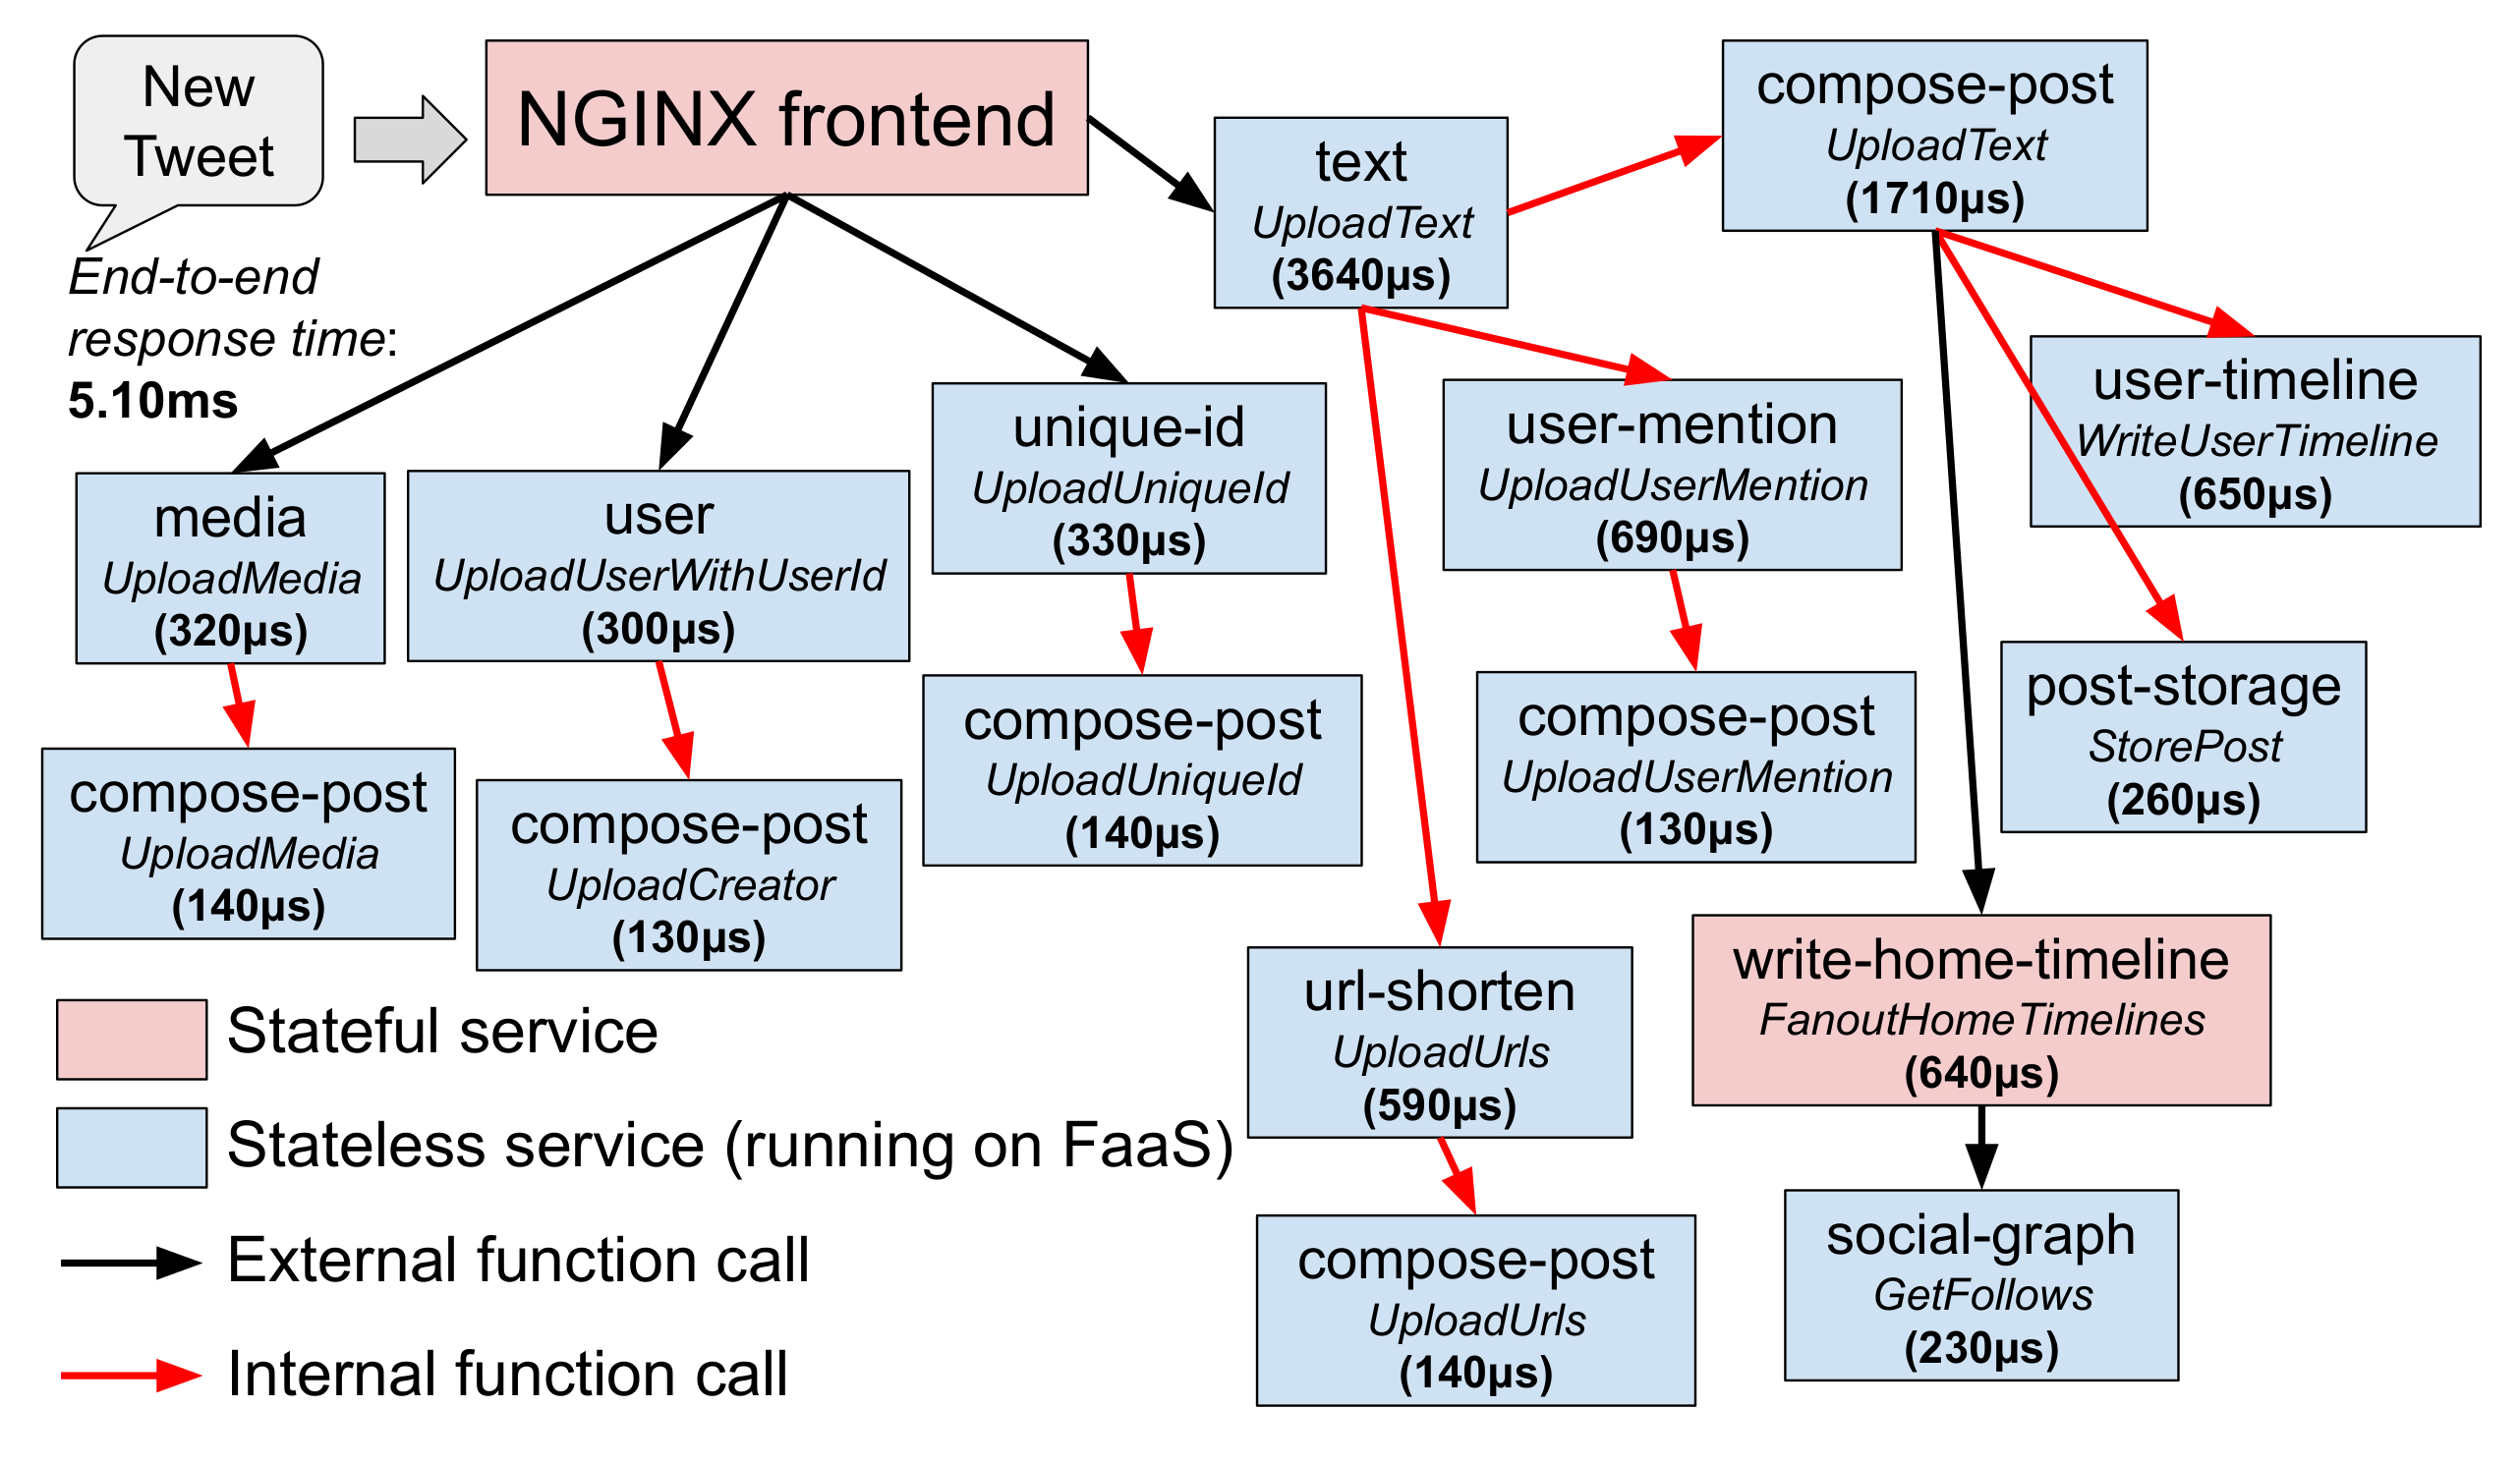
\includegraphics[width=0.8\linewidth]{res/tweet_microservice.png}
		\شرح{مثالی از زنجیره مولفه برای ارسال یک توویت (برگرفته از \مرجع{jia2021nightcore})}
	\end{figure}
\end{frame}

\begin{frame}{نیاز به توزیع‌کننده بار}
	\begin{itemize}\RTList
	\فقره در این معمار چندین خدمت‌گزار یک مولفه یکسان را اجرا می‌کنند.
	\فقره توزیع‌کننده بار تصمیم می‌گیرد که درخواست‌ها در کدام خدمت‌رسان پردازش شوند.
	\فقره هدف این است که دریافت کننده خدمات چندین خدمت‌گزار به صورت یک خدمت‌گزار مشاهده کند.
	\end{itemize}
	\begin{figure}
		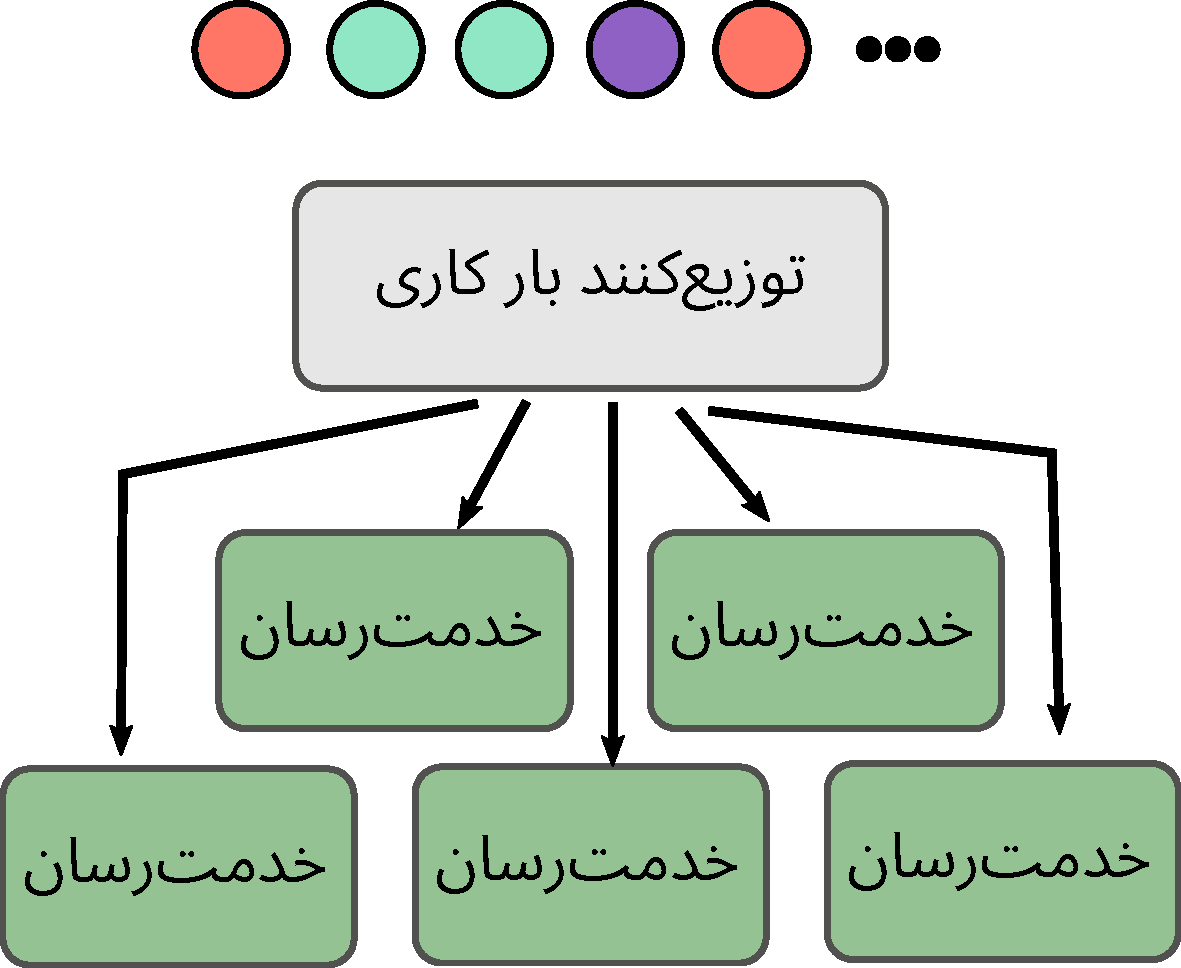
\includegraphics[width=0.4\linewidth]{res/loadbalancer.pdf}
	\end{figure}
\end{frame}

\begin{frame}{پیچیدگی زیرساخت معماری میکروسرویس}
	\mybox{چالش}{
		ایجاد و پیاده‌سازی سیستم‌های نرم‌افزاری با ویژگی‌های شرح داده شده هزینه‌بر و دارای
		چالش‌های فنی بسیاری است.
	}
\end{frame}

\begin{frame}{خدمات پردازش بدون‌میزبان}
	\begin{itemize}\RTList
	\فقره پردازش بدون‌میزبان یک چارچوب پردازش ابری است.
	
	\فقره برنامه ساز می‌تواند برنامه خود را بدون
	نیاز به فعالیت‌های اجرایی مانند تهیه و تخصیص منابع پردازشی ایجاد و اجرا کند.
	
	\فقره وظیفه مسائل مربوط به \توچشم{اتکاپذیری} و \توچشم{مقیاس‌پذیری} بر عهده ارائه دهنده خدمات است. 
	
	\فقره میزان هزینه این خدمات بر اساس
	میزان مصرف واقعی برنامه از منابع موجود محاسبه می‌شود\مرجع{kounev2021toward}.
	\end{itemize}
\end{frame}

\begin{frame}{معماری سکوی پردازش بدون‌میزبان}
	\begin{figure}[!h]
		\centering
		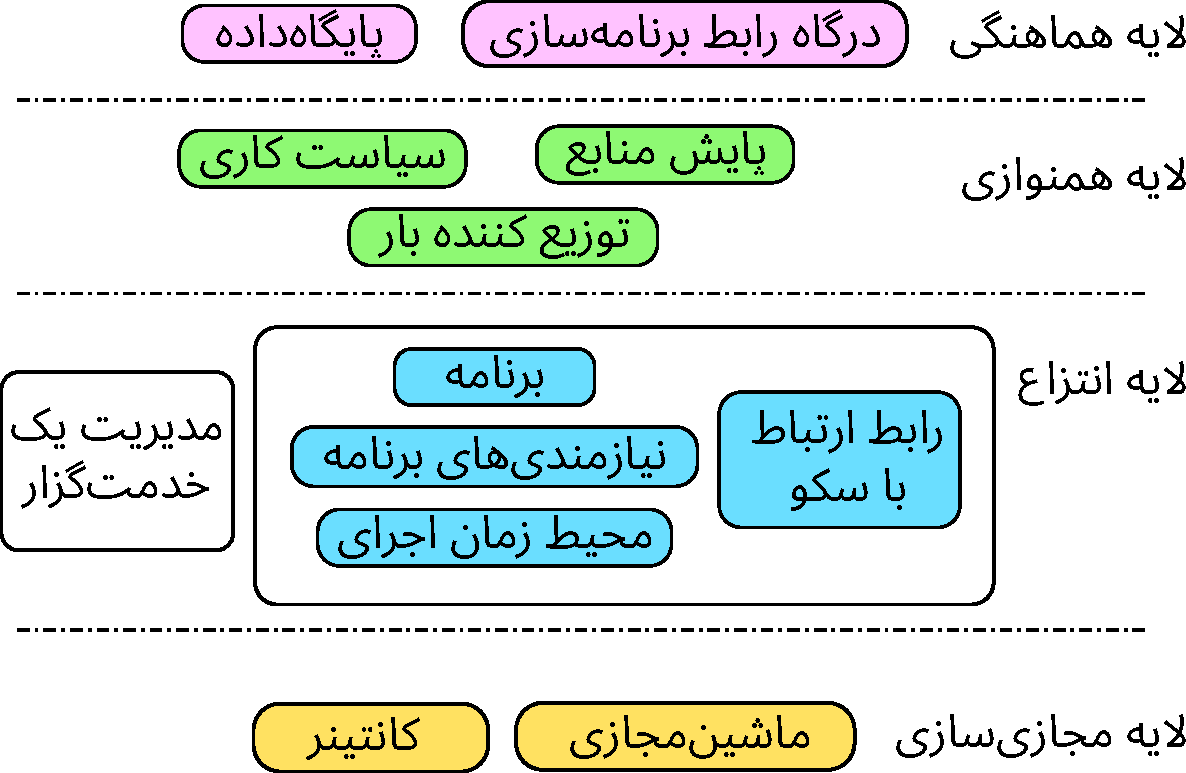
\includegraphics[width=0.5\linewidth]{res/serverless_architecture.pdf}
		\شرح{نگاه سطح بالا به لایه‌های مختلف در سکوهای پردازش بدون‌میزبان}
		\برچسب{معماریسطحبالا}
	\end{figure}
\end{frame}

\begin{frame}{ویژگی‌های برنامه‌های پردازش بدون‌میزبان}
	\begin{itemize}\RTList
	\فقره مولفه‌ها در قالب توابع مبتنی بر رخداد تعریف شده‌اند.
		
	\فقره در هنگام دریافت رخداد یک نسخه از این توابع در یک محیط زمان‌اجرا بارگیری می‌شود و رخداد را پردازش می‌کند.
	
	\فقره در طول اجرا، یک مولفه  می‌تواند دیگر مولفه‌ها را فراخوانی کند و یک زنجیره اجرا ایجاد کند.
		
	\فقره در ذات اجرای مولفه‌ها مواردی همچون \توچشم{همروندی} اجرای چندین مولفه، \توچشم{وقوع اشکال} در زمان اجرا،
		\توچشم{تلاش مجدد یک اجرا} و \توچشم{استفاده مجدد از محیط زمان اجرای} یک مولفه وجود دارد. 
		
	\فقره محیط‌های اجرا در ابتدا سرد هستند و پس از پردازش اطلاعات گرم در نظر گرفته می‌شوند.

	\فقره پس از پایان پردازش یک محیط اجرا می‌تواند بسته شود یا برای مدتی باز بماند.
			\end{itemize}
\end{frame}

%ارائه خدمات بر بستر شبکه اینترنت بخش بزرگی از عرصه پردازش در عصر حاضر را تشکیل داده است و
%فناوری‌های جدیدی مانند اینترنت اشیا و ماشین‌های خودران را امکان پذیر ساخته است. از ملزومات
%ارائه خدمات فراگیر، قابلیت مقیاس پذیری و اتکاپذیری آن است.
%تضمین این دو ویژگی با ایجاد سیستم خدماتی به صورت توزیع شده امکان‌پذیر است. 
%به همین منظور تولید کنندگان سیستم‌های نرم‌افزاری از معماری‌های توزیع شده
%مانند میکروسرویس استفاده می‌کنند.
%
%در این معماری، سیستم به مولفه‌هایی ریزدانه‌ و مستقل تقسیم شده است که با یک دیگر در
%بستر شبکه‌های کامپیوتری در ارتباط هستند. هر مولفه می‌توانند به صورت جداگانه بر روی
%تعدادی خدمت‌رسان اجرا شود. این امر انعطاف لازم را ایجاد می‌کند که در مواقع افزایش
%بار کاری با افزایش تعداد خدمت‌رسان‌ها، مولفه‌ای از سیستم که نیاز به توان بیشتر برای
%پرداز دارد مقیاس پذیرد. همچنین اگر تعدادی از خدمت‌رسان‌ها دچار اشکال شوند، در روند
%کلی خدمت‌رسانی مشکل عمده‌ای رخ نمی‌دهد و تنها شاهد کاهش توان پردازشی خواهیم بود.
%
%در این نوع از سیستم‌ها به دلیل تعدد وجود خدمت‌رسان برای مولفه‌های مختلف نیاز به یک
%توزیع کننده بار کاری میان خدمت‌رسان های موجود است. وظیفه توزیع کننده بار
%است که کل بار موجود را با توجه به سیاست از پیش تعیین شده به نحوی توزیع کند که
%از دید دریافت کننده خدمات تمام خدمت‌رسان‌ها به صورت یک خدمت‌رسان واحد مشاهده شود.
%
%ایجاد و پیاده‌سازی سیستم‌های نرم‌افزاری با ویژگی‌های شرح داده شده هزینه‌بر و دارای
%چالش‌های فنی بسیاری است. از این جهت ارائه دهندگان خدمات زیرساخت و خدمات سکو‌های
%نرم‌افزاری راهکاری با نام پردازش بدون میزبان ارائه کرده‌اند. در این روش، تولید
%کنندگان نرم‌افزار فقط بر روی ایجاد مولفه‌های خود تمرکز می‌کنند و اجزای کاربرد
%خود را با استفاده از چارچوب‌های از پیش تعیین شده پیاده سازی می‌کنند. سپس
%کدهای خود را برای اجرا به ارائه دهنده خدمات پردازش بدون میزبان ارسال می‌کنند.
%
%ارائه دهندگان خدمات پردازش بدون میزبان یک سکوی یک‌پارچه برای اجرای برنامه‌های مشتریان
%خود توسعه داده‌اند که به صورت خودکار برنامه مولفه‌های مختلف را از مشتری دریافت می‌کند و
%آن را بر روی تعدادی خدمت‌گزار اجرا می‌کند.
%وظیفه مقیاس‌پذیری و اتکاپذیری برنامه مشتری بر عهده ارائه دهنده خدمات است و توسط سکوی
%پردازش بدون میزبان به صورت خودکار اجرا می‌شود.
%
%سکو‌های پردازش بدون‌میزبان یک سطح انتزاع برای ایجاد برنامه با قابلیت مقایس‌پذیری بالا
%ارائه کرده اند. در هنگامی که بار میزان بار کاری برنامه تغییر می‌کند، این سکو با توجه
%به نیاز برنامه تعداد خدمت‌رسان‌ها را تنظیم و بار کاری را بین آن‌ها توزیع می‌کند. از این
%منظر توزیع‌بار مناسب میان خدمت‌گزارهای فعال از بخش‌های اساسی این سکوها است.
%
%با توجه به اهمیت سکو‌های پردازش بدون‌میزبان، هدف از این پروژه بررسی و ارزیابی کارایی
%این سکوها با تمرکز ویژه بر روی مولفه توزیع‌بار است. چارچوب‌های پردازش بدون‌میزبان
%باعث بروز برنامه‌هایی شده است که زمان اجرای کوتاهی دارند ولی به صورت متعدد و گسترده
%در مراکز داده اجرا می‌شوند به همین دلیل چالش‌های جدید و متنوعی ایجاد شده است.
%از چند مورد از این چالش‌های می‌توان به 
%سربار قابل توجه محیط زمان اجرا\مرجع{khatri2020potential} و یا کاهش چشمگیر کارایی زمانی
%که برنامه در ابتدای اجرای خود است\مرجع{lloyd2018serverless}.
%تمرکز این پروژه بر روی شناسایی چالش‌ها و بر طرف کردن آن‌ها با توزیع مناسب بار است.
%
%ادامه این بخش به صورتی که در ادامه می‌آید تنظیم شده است. ابتدا به معماری سیستم‌های
%بدون‌میزبان و ساختار اجرای مولفه‌ها پرداخته می‌شود.
%اهمیت سیستم‌های توزیع‌بار شرح داده می‌شود و
%درنهایت روش‌ها ارزیابی کارایی سیستم‌های تحت شبکه درون مراکز داده معرفی می‌گردد.
%
%
%\زیرقسمت{معماری سکو پردازش بدون‌میزبان}
%
%در منابع موجود، پردازش بدون‌میزبان به صورتی که در ادامه می‌آید تعریف شده است.
%این تعریف با روشن ساختن چیستی پردازش بدون‌میزبان به درک بهتر معماری سیستم های
%پردازش بدون‌میزبان کمک می‌کند.
%
%پردازش بدون‌میزبان یک چارچوب پردازش ابری است که یک مدل برنامه سازی سطح بالا
%ارائه می‌کند به نحوی که برنامه ساز می‌تواند برنامه ابری خود را بدون
%نیاز به فعالیت‌های اجرایی مانند تهیه و تخصیص منابع پردازشی ایجاد و اجرا کند.
%وظیفه مسائل مربوط به اتکاپذیری و یا تنظیم توان پردازشی با میزان نیاز برنامه
%بر عهده ارائه دهنده خدمات زیرساخت ابری است. میزان هزینه این خدمات بر اساس
%میزان مصرف واقعی برنامه از منابع موجود محاسبه می‌شود\مرجع{kounev2021toward}.
%
%\begin{figure}[!h]
%	\centering
%	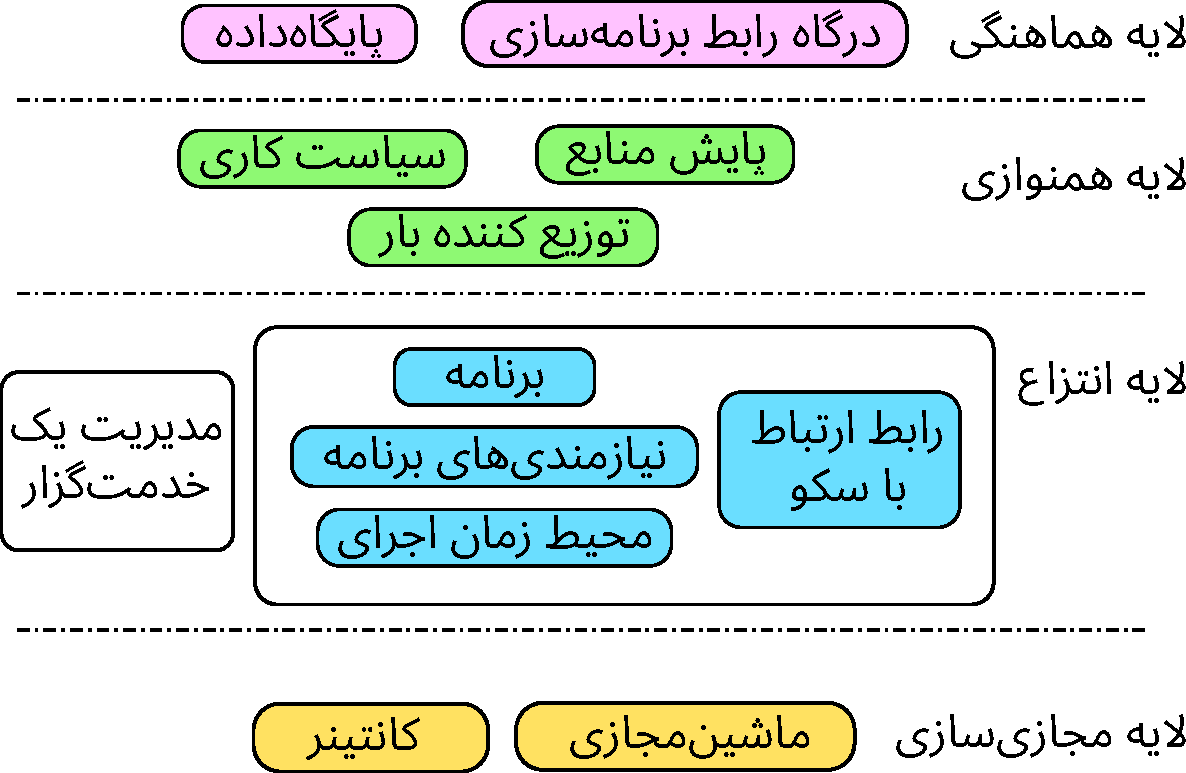
\includegraphics[width=0.5\linewidth]{res/serverless_architecture.pdf}
%	\شرح{نگاه سطح بالا به لایه‌های مختلف در سکوهای پردازش بدون‌میزبان}
%	\برچسب{معماریسطحبالا}
%\end{figure}
%
%همانطور که در شکل \رجوع{معماریسطحبالا} دیده می‌شود، معماری این سیستم‌ها به چهار لایه
%(۱) مجازی‌سازی، (۲) انتزاع، (۳) همنوازی و (۴) هماهنگی ‌تقسیم می‌شود.
%
%لایه مجازیسازی امکان ایزوله کردن برنامه‌های مختلف در حال اجرا بر روی یک سیستم را فراهم می‌کند.
%تکنولوژی‌های پر طرفدار مورد استفاده در این لایه متنوع است ولی استفاده از ماشین‌ مجازی و یا
%کانتینر در این لایه بسیار مرسوم است. لایه مجازیسازی به صورت مجزا بر روی هر خدمت‌گزار اجرا می‌شود.
%
%لایه انتزاع، امکان فراهم سازی محیط اجرای برنامه‌ها و ارتباط میان مولفه‌های مختلف را فراهم می کند.
%در هنگام دریافت یک درخواست از لایه همنوازی، محیط اجرای برنامه که شامل نیازمندی‌ها، سیستم زمان اجرا
%و محیط مجازی است، آماده می‌شود و پردازش در آن صورت می‌گیرد. همچنین اگر نیاز به برقرار ارتباط
%با مولفه‌های دیگر در همین خدمت‌رسان و یا خدمت‌رسان دیگری در مرکز داده باشد، این لایه شیوه‌نامه ارتباطی
%را مشخص می‌کند.
%
%لایه همنوازی وظیفه مقیاس‌پذیری و اتکاپذیری سیستم را دارد. این لایه بار کاری را میان خدمت‌رسان‌ها
%توزیع می‌کند. همچنین موارد مربوط به ردگیری میزان مصرف و پایش سیستم‌ هم در این لایه صورت می‌گیرد.
%
%لایه هماهنگی مواردی همچون درگاه رابط برنامه‌نویسی، پایگاه‌های داده، زیر سیستم‌های مربوط به کارهای
%توسعه و عملیات اجرایی را در بر می‌گیرد.
%
%\زیرقسمت{ساختار مولفه‌ها در پردازش بدون‌میزبان}
%\برچسب{ساختارمولفه}
%
%\begin{figure}[!h]
%	\centering
%	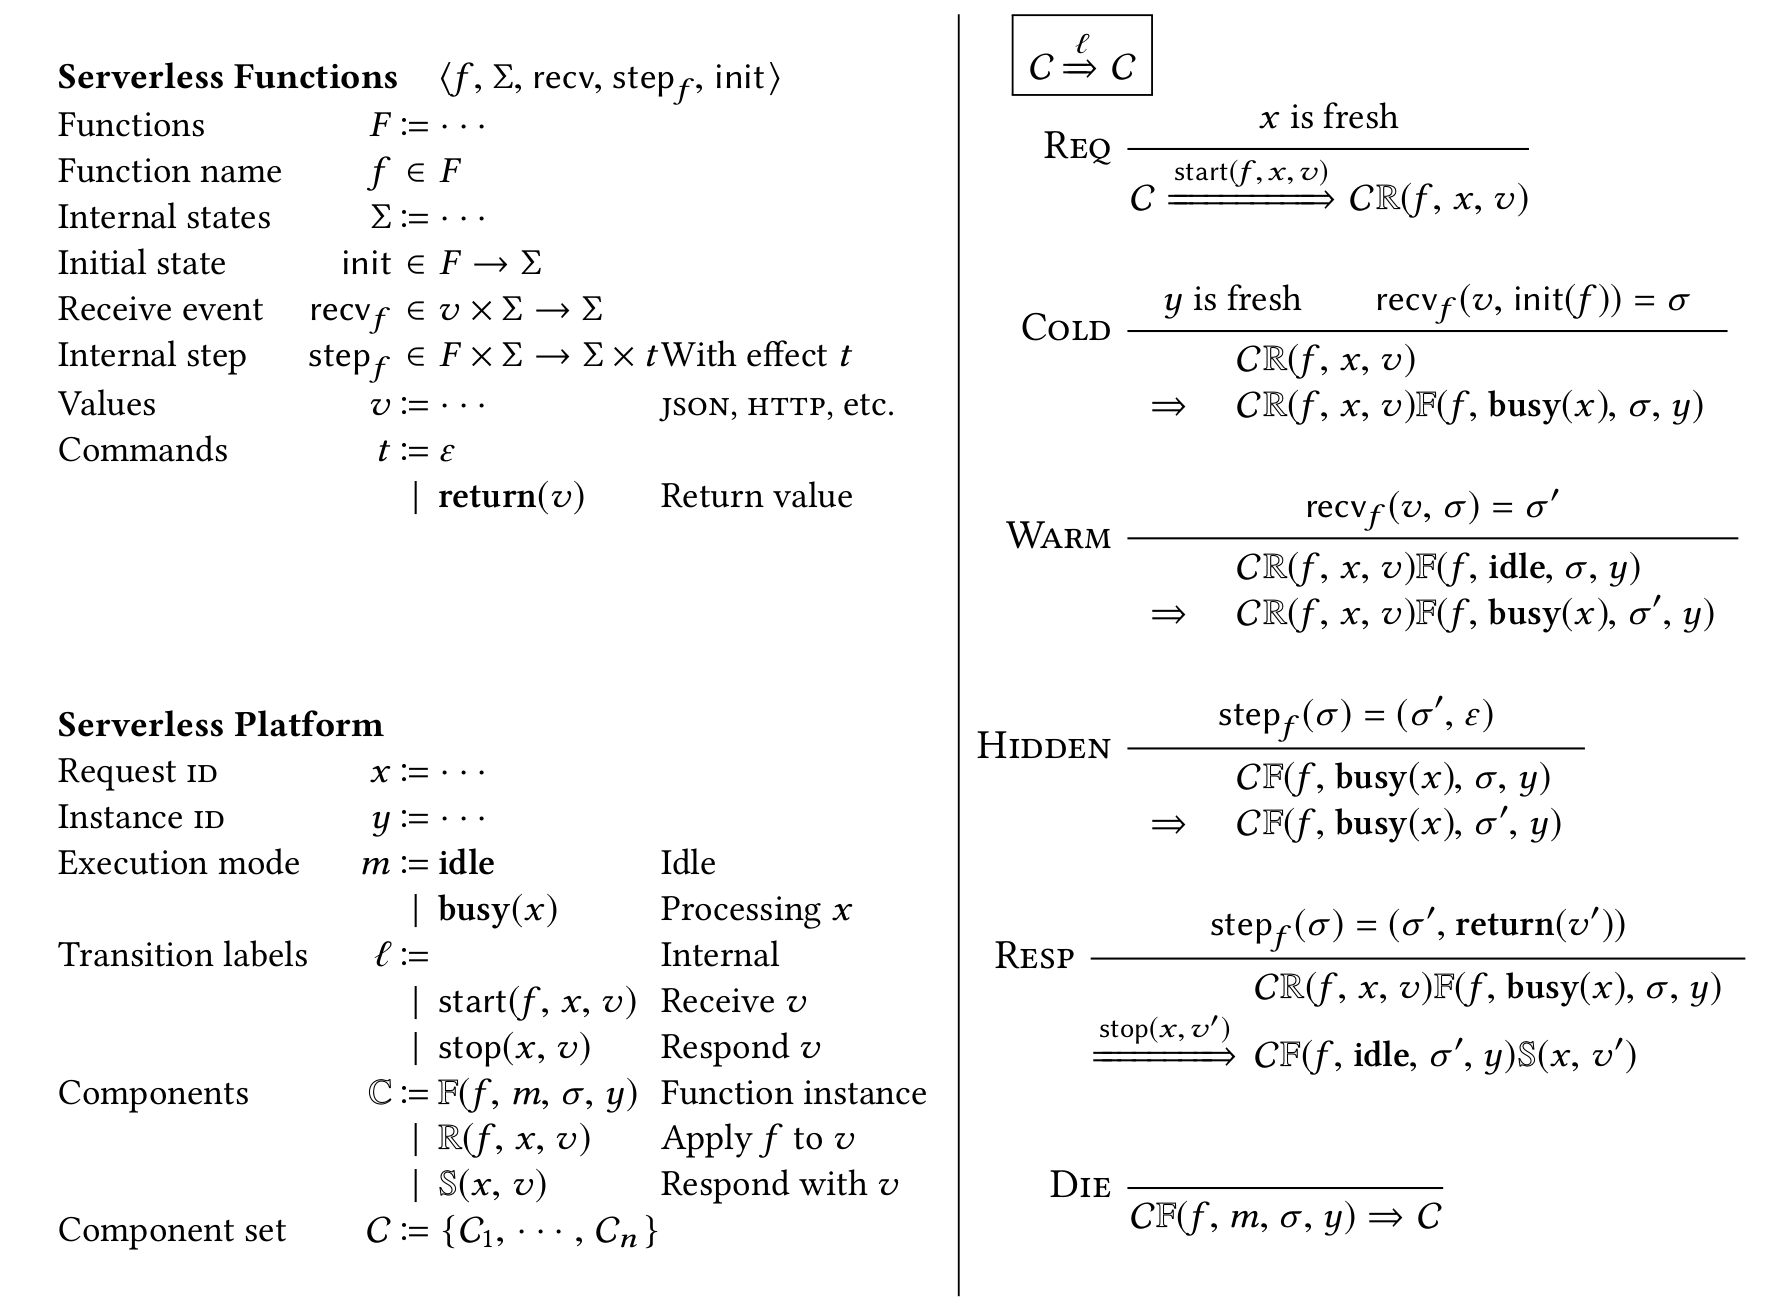
\includegraphics[width=0.9\linewidth]{res/sos.png}
%	\شرح{مدل معناشناسی ساخت‌یافته عملیاتی برای مولفه‌های پردازش بدون‌میزبان (برگرفته از \مرجع{jangda2019formal})}
%	\برچسب{سوس}
%\end{figure}
%
%ایجاد کنندگان نرم‌افزار مولفه‌های خود را در قالب توابعی که به صورت مبتنی بر رخداد تعریف شده‌اند،
%تشکیل می‌دهند. در هنگام دریافت رخدادهای مورد نظر یک مولفه، یک نسخه از این توابع در یک محیط زمان اجرا
%بارگیری می‌شود و رخداد را پردازش می‌کند. در طول اجرا، یک مولفه  می‌تواند دیگر مولفه‌ها را فراخوانی کند
%و در نتیجه یک زنجیره اجرا از مولفه‌ها را تشکیل دهد.
%
%در ذات اجرای مولفه‌ها مواردی همچون همروندی اجرای چندین مولفه، وقوع اشکال در زمان اجرا،
%تلاش مجدد یک اجرا و استفاده مجدد از محیط زمان اجرای یک مولفه وجود دارد. تمام این موارد
%باعث پیچیدگی مفهومی توابع مورد نظر می‌شود. برای درک بهتر از ساختار برنامه سازی سیستم‌های
%بدون‌میزبان مدل معناشناسی ساخت‌یافته عملیاتی در شکل \رجوع{سوس} ارائه شده است\مرجع{jangda2019formal}.
%
%برای هر مولفه $f$ می‌تواند در هر زمان یک درخواست بیاید که به آن یک شناسه منحصر به فرد $x$ نسبت داده شده‌است
%(قاعده $Req$).
%در خواست دریافت شده یا منجر به ایجاد یک محیط اجرا جدید می‌شود (قاعده $Cold$) و یا در یک محیط اجرای از پیش
%آمده ادامه پردازش می‌شود (قاعده $Warm$). مراحل اجرای پردازش از دید این مدل پنهان است (قاعده $Hidden$).
%در نهایت پس از ایجاد پاسخ پردازش (قاعده $Resp$) محیط پردازش آزاد می‌شود و می‌تواند دوباره مورد استفاده قرار 
%بگیرد و یا اینکه محیط اجرا بسته می‌شود (قاعده $Die$).
%
%
%\زیرقسمت{چالش‌های توزیع‌بار در سکو‌های پرداز بدون‌میزبان}
%
%توزیع‌بار کاری میان خدمت‌گزاران مختلف از این جهت حائز اهمیت است که زمان‌بندی اجرای برنامه‌ها،
%تعداد خدمت‌گزاران فعال برای پردازش و اعمال سیاست‌های تضمین کیفیت خدمات از جمله وظایف آن است.
%
%برنامه‌‌هایی که در سکو پردازش بدون‌میزبان اجرا می‌شوند نیازهای متنوعی دارند. یک مطالعه نشان می‌دهد
%که اندازه برنامه‌ها از یک مولفه تا صدها مولفه متغییر است و زمان اجرای هر کدام از مولفه در بازه‌ی
%کمتر از یک ثاینه تا چندین دقیقه تغییر می‌کند \مرجع{tariq2020sequoia}.
%
%در هنگام دریافت یک رخداد، توزیع کننده بار باید ابتدا با توجه نوع رخداد فرآیند زمانبندی را انجام
%دهد و سپس با توجه به حالت خدمت‌گزارهای مرکز داده، درخواست را به یک خدمت‌گزار تحویل دهد. دو مسئله
%در این موضوع وجود دارد. اول اینکه هر کدام رخداد در چه زمانی به خدمت‌گزار ارسال شود. دوم آنکه
%درخواست به کدام خدمت‌گزار ارسال شود.
%
%زمان ارسال درخواست به خدمت‌گزار، برای تضمین کیف خدمات بسیار اثر گذار است. از طرفی عملیات
%زمانبندی نیاز به حافظه برای میانگیری درخواست‌های در حال انتظار دارد. اگر حافظه تخصیص داده
%شده پر شود آنگاه درخواست‌های  مازاد ارسال شده طرد می‌شوند.
%
%انتخاب خدمت‌گزاری که قرار است درخواست را پردازش کند نیز از اهمیت بالایی برخوردار است. اگر
%نیاز باشد که یک محیط اجرای جدید روی خدمت‌گزار ایجاد شود، این عملیات زمانبر خواهد بود.
%همچنین کارایی‌ محیط اجرایی که به تازگی ایجاد شده است (در حالت سرد است) از اجرای درخواست در یک
%محیط که از قبل وجود داشته شده است (در حالت گرم است) می‌تواند تا ۱۵ برابر کندتر باشد\مرجع{lloyd2018serverless}.
%
%
%\زیرقسمت{ارزیابی کارایی مراکز داده}
%
%برای ارزیابی کارایی سیستم‌های مراکز داده روش های گوناگونی وجود دارد. در این پروژه بر روی
%تئوری صف تمرکز شده است.
%
%\زیرزیرقسمت{تئوری صف}
%
%\begin{figure}[!h]
%	\centering
%	
\includegraphics[width=0.3\linewidth]{res/queue.png}
%	\شرح{نمایش یک صف در مدل تئوری صف}
%	\برچسب{صف}
%\end{figure}
%
%در تئوری صف یک واحد پردازش به صورتی که در شکل \رجوع{صف} مشاهده می‌شود نمایش داده می‌شود.
%در این مدل با دانستن توزیع احتمالاتی رخداد‌ها و نرخ ورود و نرخ پردازش با استفاده از روش‌های تحلیلی مواردی از جمله 
%زمان انتظار و گذردهی سیستم محاسبه می‌شود. از چالش‌های استفاده این مدل برای سکوهای پردازش بدون‌میزبان تغییر
%تعداد خدمت‌گزاران، نرخ ورود و نرخ خروج سیستم به صورت پیوسته است. با ایجاد یک محیط اجرای جدید در واقع یک 
%صف جدید به مدل اضافه شده است و چون محیط اجرا در ابتدا در حالت سرد قرار دارد پس نرخ سرویس‌ دهی پایینی دارد
%با گرم شدن محیط اجرا، نرخ سرویس دهی افزایش پیدا می‌کند. در هنگامی که یک محیط اجرا بسته می‌شود یک صف از مدل
%حذف می‌شود. این تغییرات محاسبات تحلیلی را با چالش‌های فراوان همراه می‌سازد.
%
%یک روش دیگر برای محاسبه کارایی این سیستم‌ها استفاده از شبیه‌سازی است. با ایجاد مدل تئوری صف می‌توان محیط‌های شبیه‌سازی
%را با پارامترهای معین ایجاد کرد و با اجرای شبیه‌سازی برای تعداد زیادی از درخواست‌ها و به صورت مکرر می‌توان کارایی
%سیستم را ارزیابی کرد.